                                                        %%%%%%%%%%%%%%%%%%%%%%%%%%%%%%%%%%%%%%%%%%%%%%%%%%%%%%%%%%%%
%%% ELIFE ARTICLE TEMPLATE
%%%%%%%%%%%%%%%%%%%%%%%%%%%%%%%%%%%%%%%%%%%%%%%%%%%%%%%%%%%%
%%% PREAMBLE 
\documentclass[9pt,lineno]{elife}
% Use the onehalfspacing option for 1.5 line spacing
% Use the doublespacing option for 2.0 line spacing
% Please note that these options may affect formatting.
% Additionally, the use of the \newcommand function should be limited.


\usepackage{lipsum} % Required to insert dummy text
\usepackage[version=4]{mhchem}
\usepackage{siunitx}
\usepackage{comment}
\usepackage{tikz}
\usetikzlibrary{bayesnet}
\DeclareSIUnit\Molar{M}

% \makeglossaries

\newglossaryentry{n}{
    name=\ensuremath{n},
    description={target site}
}

%%%%%%%%%%%%%%%%%%%%%%%%%%%%%%%%%%%%%%%%%%%%%%%%%%%%%%%%%%%%
%%% ARTICLE SETUP
%%%%%%%%%%%%%%%%%%%%%%%%%%%%%%%%%%%%%%%%%%%%%%%%%%%%%%%%%%%%
\title{Bayesian analysis of the colocalization single molecule image data}

\author[1*]{Yerdos A. Ordabayev}
\author[1,2\authfn{1}\authfn{3}]{Larry Friedman}
\author[2\authfn{1}\authfn{4}]{Douglas L. Theobald}
\author[2*]{Jeff Gelles}
\affil[1]{Brandeis University}
\affil[2]{Institution 2}

\corr{email1@example.com}{FMS}
\corr{email2@example.com}{FS}

\contrib[\authfn{1}]{These authors contributed equally to this work}
\contrib[\authfn{2}]{These authors also contributed equally to this work}

\presentadd[\authfn{3}]{Department, Institute, Country}
\presentadd[\authfn{4}]{Department, Institute, Country}
% \presentadd[\authfn{5}]{eLife Sciences editorial Office, eLife Sciences, Cambridge, United Kingdom}


%%%%%%%%%%%%%%%%%%%%%%%%%%%%%%%%%%%%%%%%%%%%%%%%%%%%%%%%%%%%
%%% ARTICLE START
%%%%%%%%%%%%%%%%%%%%%%%%%%%%%%%%%%%%%%%%%%%%%%%%%%%%%%%%%%%%

\begin{document}

\maketitle

\begin{abstract}
Please provide an abstract of no more than 150 words. Your abstract should explain the main contributions of your article, and should not contain any material that is not included in the main text.
\end{abstract}


\section{Introduction}

A central concern of modern biology is understanding at the molecular level the chemical and physical mechanisms by which protein and nucleic acid macromolecules  perform essential cellular functions.  The operation of many such macromolecules requires that they work not as isolated molecules in solution but as components of dynamic molecular complexes that self-assemble and change structure and composition as they function.  For more than  two decades, scientists have successfully explored the molecular mechanisms of many such complex and dynamic systems using multi-wavelength single molecule fluorescence methods such as smFRET (single-molecule fluorescence resonance energy transfer) \citep{Roy2008-fo} and single-molecule co-localization methods like CoSMoS (co-localization single molecule spectroscopy) \citep{Larson2014-os, Van_Oijen2011-ig}.

In its simplest implementation, CoSMoS is a technique to visualize transient interactions between individual molecules.  Dye-labeled protein or nucleic acid target molecules are immobilized on a slide surface and TIRF (total internal reflection fluorescence) microscopy is employed to detect co-localizations between those targets and other dye-labeled molecules that might bind those targets during a biochemical reaction.  The CoSMoS method has been used for elucidating the mechanisms of complex biochemical processes \textit{in vitro}. Examples include cell cycle regulation \citep{Lu2015-eu}, ubiquitination and proteasome-mediated protein degradation \citep{Lu2015-jq}, DNA replication \citep{Geertsema2014-bt,Ticau2015-ib}, transcription \citep{Zhang2012-no,Friedman2012-if,Friedman2013-sf}, micro-RNA regulation \citep{Salomon2015-kq}, pre-mRNA splicing \citep{Shcherbakova2013-bi, Krishnan2013-fy, Warnasooriya2014-ls}, ribosome assembly \citep{Kim2014-zc}, translation \citep{Wang2015-tt,Tsai2014-mi,OLeary2013-wo}, signal recognition particle-nascent protein interaction \citep{Noriega2014-vj}, and cytoskeletal regulation \citep{Smith2013-qj,Breitsprecher2012-mj}. CoSMoS is extensively used by labs that specialize in the technique and is increasingly being adopted by non-specialist labs as well. With the availability of good commercial TIRF microscopes, data analysis methodology is a major challenge in adoption and use of the CoSMoS technique.

Analysis of CoSMoS data is an intrinsically challenging and time-consuming problem. Although CoSMoS images are conceptually simple -- they consist only of diffraction-limited fluorescent spots collected in several wavelength channels -- efficient analysis of the images, reliable extraction of kinetic data, and fitting to model biochemical mechanisms are inherently challenging for several reasons. First, the number of photons emitted by a single fluorophore is limited by fluorophore photobleaching. Consequently, in many CoSMoS experiments one must work at the lowest feasible excitation power in order to maximize the duration of experimental recordings and to capture relevant kinetics. Achieving higher time resolution divides the number of emitted photons between a larger number of images. The required concentrations of fluorescently tagged molecules can sometimes create significant background noise \citep{Peng2018-ge, Van_Oijen2011-ig}, even with zero-mode waveguide instruments \citep{Chen2014-jd}. These technical difficulties result in CoSMoS images that frequently have low signal-to-noise (S/N) ratios, making discrimination of real fluorescent spots from noise a major challenge. Second, there are transient non-specific interactions of the binder molecule with the surface of the microscope slide, and these non-specific interactions can give rise to both false positive and false negative detections. Additional measurements and modeling of these non-specific surface interactions must be employed to avoid errors in derived kinetic parameters or inferred mechanisms.

All of the current CoSMoS analysis methods involve a two-step process. In the first co-localized spot detection step, binary information at each time point about whether a binder molecule fluorescence spot is observed at the image position of a target molecule is obtained. In the second step, kinetic parameters are extracted from the on- and off- dwell time distributions. Some spot detection methods are based on integrating the binder fluorescence intensity over small regions of the image (typically squares $\sim$0.4 $\mu$m on a side) centered on the location of the target molecule, and then using crossings of set intensity threshold(s) to score binder molecule arrival and departure. For reasons described in detail elsewhere \citep{Friedman2015-nx}, these approaches are both imprecise and inaccurate, particularly when applied to the low S/N images often used. A fundamental problem with these methods is that they rely on the integrated intensity and thus discard spatial information contained in the images that can and should be used to objectively inform decisions about spot presence.

More recent spot detection methods are based on extracting quantitative features of the spot (e.g., intensity profile, size, shape, and distance to target) from the 2-D image and then identifying spots using manually chosen thresholds for these parameters \citep{Friedman2015-nx, Smith2019-yb}. These image analysis based methods are more accurate than previous approaches in part because they make use of information contained in the 2-D images that are disregarded when only the integrated intensity is used \citep{Friedman2015-nx}. While these methods greatly improve CoSMoS data analysis, they nevertheless suffer from significant deficiencies. First, current methods require subjective choice of user-set thresholds for spot amplitude, diameter and proximity. These settings significantly affect error rates and no objective method to select them currently exists, making the approach non-robust and overly complicated. Second, it is unsatisfying from a theoretical perspective that existing analysis methods are performed in multiple step with a loss of information about the uncertainties at each step of the analysis. Spot detection is performed on the extracted features of the spot and not the raw 2-D images themselves. Furthermore, spot detection step produces only a binary output (spot present or absent); they do not output the probability of spot presence in marginal images, a critical feature in the analysis of low S/N data. Kinetic analysis, in turn, is based on the binary output of the spot detection step, further reducing the amount of information transmitted from the raw images. Third, it is nontrivial to incorporate prior knowledge (e.g., co-localization accuracy, size of the spot, frequency of non-specific binding) into these analysis methods.

To solve these problems we adopt a Bayesian inference approach which provides a natural means to combine prior information with data in a rigorous statistical framework. Bayesian inference uses Bayes' theorem to provide a probability distribution for unobserved model parameters conditional on observed data. We define a probabilistic generative model which can be interpreted as a causal process that produces the observed data. In our case observed data corresponds to an image at a target site (matrix of pixel intensities). The observed images are generated according to the likelihood function (noise model) for different settings of latent variables such as background intensity, number of spots in the image, position, shape, and intensity of each individual spot. The latent variables, in turn, are sampled from prior distributions. Prior distributions can be used to embed our knowledge into the model such as the distribution of the position of the spot depending whether it is on-target of off-target spot. Prior distributions can also represent global parameters of the model as in the case with the average probability of observing a spot in the image.

In this article, we present Bayesian approach for analysis and interpretation of CoSMoS data. Our new method: 1) provides uncertainties for all of the model parameters including a spot probability estimate for each image (not merely a Boolean spot/no spot classification) 2) maximizes extraction of useful information from data (particularly at the low S/N inherent to many CoSMoS experiments) by analyzing raw images, not just fluorescence intensities; 2) defines a unified probabilistic model which allows one to directly infer model parameters from CoSMoS image data; 3) explicitly models non-specific interactions of the binder molecule with the surface which allows to jointly analyze negative control dataset; 4) uses Gamma distribution as a more realistic intensity noise model rather than Gaussian distribution; 5) has a flexible framework that can naturally be extended to kinetic models and multi-wavelength analysis. Our new analysis method will increase the accessibility of the CoSMoS method to investigators that have important biological problems to solve but are not able to develop their own data analysis methods or to reliably use the current data analysis approaches which require parameter tweaking. The method developed here eliminates this dependence on subjective parameter adjustments and includes built-in tools for statistical assessment of the validity of the results as essential steps in the analysis process.

\section{Results}

\subsection{Multi-wavelength single-molecule co-localization (CoSMoS) methods}

We aim to improve methods for elucidating the molecular mechanisms of biochemical processes in vitro using multi-wavelength single-molecule fluorescence colocalization microscopy. For brevity, we call this experimental method CoSMoS (“colocalization single-molecule spectroscopy”). The key features of a CoSMoS experiment include: 1) One species of fluorescently labeled molecule (called the “target”) is tethered to the surface. Targets are immobilized at a surface density sufficiently low that the mean nearest-neighbor distance is large relative to the point-spread function (i.e., the diffraction-limited spot size) of the microscope. 2) Molecules, each species labeled with a different dye color, are added to the solution over the surface, typically at concentrations < 1 $\mu$M. When these “binder” molecules are freely diffusing in solution, they are invisible in TIRF. In contrast, when they are bound to the target, single binder molecules are detected as discrete fluorescent spots (Figure 1). The combination of features 1 and 2 means that formation of an individual binder-target complex is detected as spot appearance; dissociation of a binder-target complex is detected as spot disappearance \citep{friedman_viewing_2006, friedman_cosmos_analysis_2015}.

A representative CoSMoS experiment is illustrated by the example in Figure 1. In this experiment, we labeled the NusG protein with an orange dye. We then tethered to a microscope slide blue-dye-labeled DNA molecules at very low surface density (so that each molecule is resolved as a separate fluorescent spot) and observed real-time binding and dissociation of the other labeled molecules during the transcription process and its regulation.

\begin{figure}
\includegraphics[width=\linewidth]{fig}
\caption{A text-width example.}
\label{fig:view}
%% If the optional argument in the square brackets is "none", then the caption *will not appear in the main figure at all* and only the full caption will appear under the supplementary figure at the end of the manuscript.
\figsupp[Shorter caption for main text.]{This is a supplementary figure's full caption, which will be used at the end of the manuscript.}{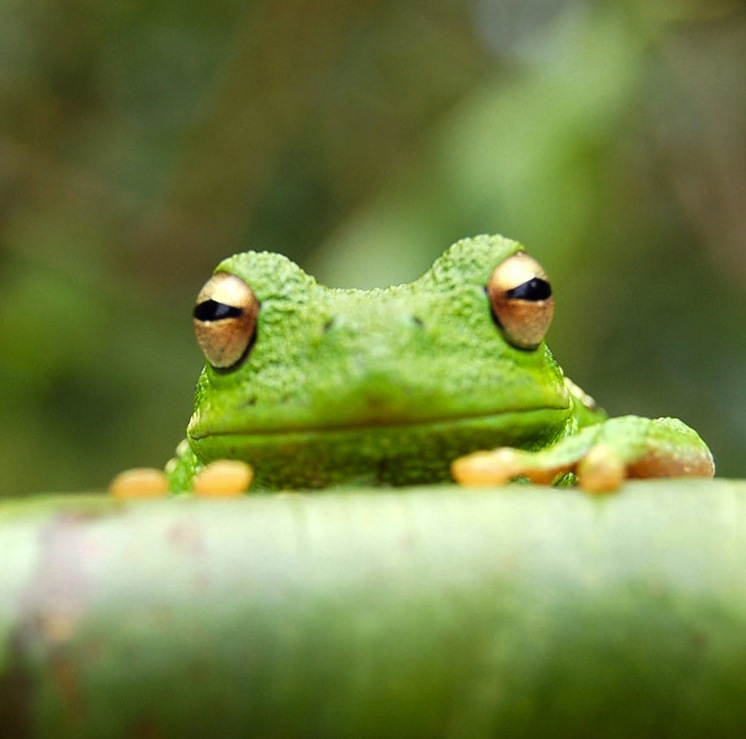
\includegraphics[width=6cm]{frog}}\label{figsupp:sf1}
\figsupp{This is another supplementary figure.}{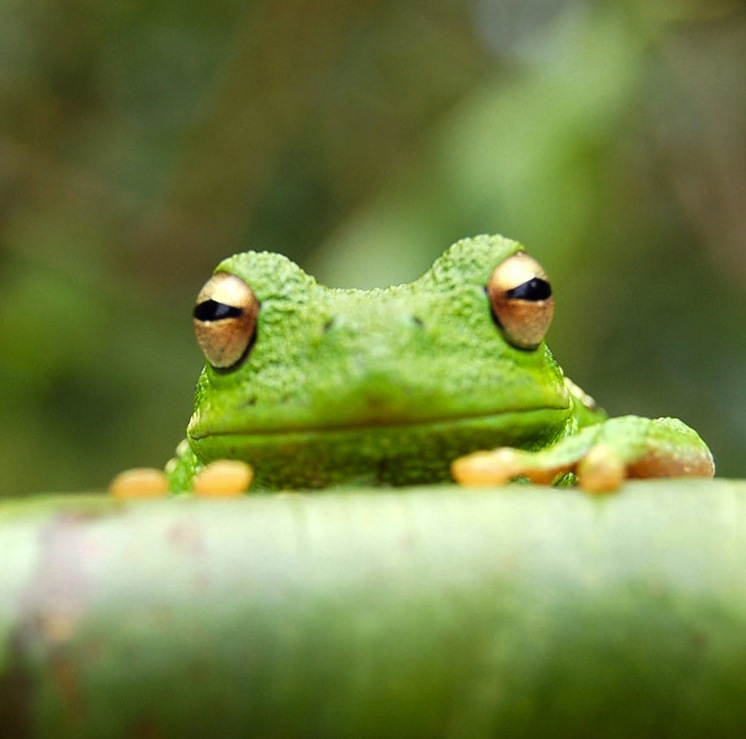
\includegraphics[width=6cm]{frog}}
\videosupp{This is a description of a video supplement.}\label{videosupp:sv1}
\figdata{This is a description of a data source.}\label{figdata:first}
\figdata{This is another description of a data source.}\label{figdata:second}
\end{figure}

\subsection{Comparison of Bayesisan method with heuristic spot thresholding}

We have done two types of performance comparison between the Bayesian method and the heuristic spot thresholding method. For the first performance comparison, a series of simulated data sets was constructed for a range of signal-to-noise values. For each S/N, a set of images with and without a 2-D Gaussian spots bound at the target and off-target were randomly generated. Intensity noise was generated using Gamma distribution to all simulated images.

Each data set was analyzed by both the Bayesian method and the heuristic spot thresholding algorithm (e.g., Figure 2, left). By comparison with the known “true” identities of the images, the accuracy of the resulting classifications was judged using a variety of specialized statistics for binary classification data, including true and false positive rates, true and false negative rates, and the Matthews Correlation Coefficient (MCC) \citep{fawcett_introduction_2006, matthews_comparison_1975}. The MCC statistic is widely regarded as a single overall, balanced measure which is meaningful even when the classes are of very different sizes. The MCC corresponds to the Pearson correlation coefficient between the estimated and “true” binary classifications. MCC=+1 represents a perfect prediction, MCC=0 a perfectly random prediction, and MCC=-1 indicates maximal disagreement between truth and estimation.

In a second comparison, images from real (i.e., not simulated) experimental data recordings were analyzed (Figure 3). Over a range of S/N, the Bayesian method gave image classification accuracy (as quantified by the MCC) similar to (or possibly better than) the heuristic spot thresholding algorithm The Bayesian method performs as well as the best existing CoSMoS data analysis method. Furthermore, Bayesian method achieves this performance automatically, with no adjustable parameters whatsoever, unlike the heuristic spot picker which attains this level of performance only after careful subjective trial-and-error manual adjustment of its three threshold parameters, a process that must be repeated tediously for each data set analyzed. Finally, our new Bayesian method produces a spot probability estimate for each image (not merely a Boolean spot/no spot determination) that can be used to inform subsequent kinetics calculations based on the results (e.g., the HMM analysis).

\subsection{Probabilistic modeling based on fundamental statistical analysis of data and priors}

To solve the problems with existing CoSMoS data analysis methods identified above, we have developed a new image-analysis-based approach that is accurate, objective, and built on a rigorous statistical approach to the CoSMoS image analysis problem. This TIBSD method is based on probabilistic modeling methodology. Bayesian model is a statistical model where probability is used to represent all uncertainty within the model, both for observed and hidden quantities in a system of interest. Bayes' theorem allows to perform inference on hidden variables given the observed data. The proposed first use of these methods for CoSMoS allows straightforward estimates of the uncertainty for estimated model parameters and rigorous quantitative testing of alternative image, noise, and kinetic models. “Time-independent” in the name TIBSD indicates that we ignore the time dimension of the recording -- the order of the images is arbitrary and does not affect the model, as each image is considered statistically independent of the others. We note that this time-independent method can naturally be extended into a time-dependent approach to both more accurately analyze the images and to directly obtain information about molecular kinetic mechanisms.  The proposed methods will eliminate the need for subjective image inspection and minimize the manual work required for CoSMoS data analysis.

\subsection{Time-independent Bayesian Spot Discrimination (TIBSD) method for analysis of CoSMoS data}

Unlike standard analysis methods for CoSMoS and single molecule FRET (smFRET), which are based on scalar intensity measurements derived from integration of emission in image regions of interest, our model fully uses information contained in the raw two-dimensional microscope images. The value of image data is proven in previous studies (Larry, Grunwald). To analyze the CoSMoS image classification problem within a Bayesian framework, one must define ideal image shapes for each class (image model) and choose a likelihood function for the observed data (noise model).

\subsubsection{Image classification}

The CoSMoS data set consists of a set of images where we have $N$ target sites ($n \in \{1,\dots,N\}$) each consisting of a series of $F$ different images in a recording ($f \in \{1,\dots,F\}$) (a “recording”). In each image, a binder molecule is either present on the single target molecule or absent. In addition, we explicitly model off-target binding of binder molecule. For simplicity  we assume that experimental conditions and image size were chosen so that at most only two spots ($K=2$) can exist in one image ($m_{nfk} \in \{ 0,1 \}$ -- existence indicator of the $k$-th spot). We treat the image classification problem as a data association problem by introducing an index variable for the on-target spot ($\theta_{nf} \in \{ 0,1,\dots,K \}$) where 0 means that on-target molecule is absent.

\subsubsection{Image model}

In the TIBSD method, we model the observed image data as a mixture of background image and “spot” images of binder molecules superimposed on background image. In particular, background image is modeled as a constant average background intensity $b_{nf}$; each spot image (2D point spread function) is modelled as an ideal (i.e., noiseless) 2-D Gaussian spot with integrated scalar intensity $h_{nfk}$ centered at ($x_{nfk}, y_{nfk}$). Each image is represented as a matrix (2D-array) $\mu^D_{nfij}$ of $P \times P$ pixels ($i,j \in \{1,\dots,P\}$). 

\textbf{\begin{equation*}
    \mu^{D}_{nfij} = b_{nf} + \sum_{k=1}^{K} \dfrac{m_{nfk}h_{nfk}}{2 \pi w^2_{nfk}} \exp{\left ( -\dfrac{(i-x_{nfk})^2 + (j-y_{nfk})^2}{2w^2_{nfk}} \right)}
\end{equation*}}

\subsubsection{Noise model}

 We use Gamma distribution as a noise model which is more flexible than Gaussian noise and can better approximate Poissonian camera noise. Scale parameter [add the variable name here?] of the Gamma distribution can be interpreted as a camera gain. Thus, the likelihood for the observed image can be expressed as:
 
 \begin{equation*}
     p(D_{nf}|\mu^D_{nfij},gain) = Gamma(D_{nf}|\mu^D_{nfij}/gain,1/gain)
 \end{equation*}

\subsubsection{Prior knowledge of colocalization accuracy}

Prior knowledge of colocalization accuracy can be directly incorporated into our model as priors for the center of the spot. On-target spots are localized around the target molecule within the experimentally determined accuracy and off-target spots are uniformly distributed within the image:

\begin{equation*}
    x_{nfk} \sim
\begin{cases}
    Beta^{\prime}(x_{nfk}|\mu^x=0,\nu^x_{prox}),& \text{if } \theta = k\\
    Beta^{\prime}(x_{nfk}|\mu^x=0,\nu^x_{flat}),& \text{otherwise}
\end{cases}
\end{equation*}

\begin{equation*}
    y_{nfk} \sim
\begin{cases}
    Beta^{\prime}(y_{nfk}|\mu^y=0,\nu^y_{prox}),& \text{if } \theta = k\\
    Beta^{\prime}(y_{nfk}|\mu^y=0,\nu^y_{flat}),& \text{otherwise}
\end{cases}
\end{equation*}


%\subsection{Image analysis, probabilities not binary classification}

%Expresses uncertainty. Allows downstream analysis. 

%\subsection{Flexible framework. Can select and use different models depending on the experiment}

%\subsubsection{Ability to jointly analyze different experimental conditions}

%\subsubsection{Models easily expandable to incorporate other data features}

\subsection{Software and hardware implementation}

The proposed research will provide more efficient ways to analyze large CoSMoS data sets. Technological developments such as faster, larger cameras \citep{huang_particle_nodate}, availability of fluorescent dyes with dramatically improved photostability (which increase the amount of data from a single experiment), and microscopes that efficiently collect single-molecule data at more wavelengths simultaneously \citep{friedman_viewing_2006} have all increased the sizes of CoSMoS datasets. Gelles lab studies of transient molecular binding events at high frame rates have produced >1 TB image data per experiment. Increasing data set sizes make it infeasible to use existing analytical methods. The code for the model and variational inference algorithm is written using Pyro probabilistic programming language. Pyro uses Pytorch as a backend for automatic differentiation and efficient computation of parallelizable vector-math operations on graphics processing units (GPUs). Our program is open-source and can be downloaded from the github repository.

\begin{comment}
\begin{table}[bt]
\caption{\label{tab:example}Automobile Land Speed Records (GR 5-10).}
% Use "S" column identifier to align on decimal point 
\begin{tabular}{S l l l r}
\toprule
{Speed (mph)} & Driver          & Car                        & Engine    & Date     \\
\midrule
407.447     & Craig Breedlove & Spirit of America          & GE J47    & 8/5/63   \\
413.199     & Tom Green       & Wingfoot Express           & WE J46    & 10/2/64  \\
434.22      & Art Arfons      & Green Monster              & GE J79    & 10/5/64  \\
468.719     & Craig Breedlove & Spirit of America          & GE J79    & 10/13/64 \\
526.277     & Craig Breedlove & Spirit of America          & GE J79    & 10/15/65 \\
536.712     & Art Arfons      & Green Monster              & GE J79    & 10/27/65 \\
555.127     & Craig Breedlove & Spirit of America, Sonic 1 & GE J79    & 11/2/65  \\
576.553     & Art Arfons      & Green Monster              & GE J79    & 11/7/65  \\
600.601     & Craig Breedlove & Spirit of America, Sonic 1 & GE J79    & 11/15/65 \\
622.407     & Gary Gabelich   & Blue Flame                 & Rocket    & 10/23/70 \\
633.468     & Richard Noble   & Thrust 2                   & RR RG 146 & 10/4/83  \\
763.035     & Andy Green      & Thrust SSC                 & RR Spey   & 10/15/97\\
\bottomrule
\end{tabular}

\medskip 
Source: \url{https://www.sedl.org/afterschool/toolkits/science/pdf/ast_sci_data_tables_sample.pdf}

\tabledata{This is a description of a data source.}

\end{table}
\end{comment}

%\section{Discussion}

\lipsum[9]

\section{Methods}

\subsection{CoSMoS Dataset}

The CoSMoS data set consists of a set of images where we have $N$ target sites ($n \in \{1,\dots,N\}$) each consisting of a series of $F$ different images in a recording ($f \in \{1,\dots,F\}$) (a “recording”). Each image is represented as a matrix (2D-array) of $P \times P$ pixel intensities ($i,j \in \{1,\dots,P\}$). We denote entire data set as a multi-dimensional array $D$ and the value of a specific pixel intensity as $D_{nfij}$.

\subsection{Generative probabilistic model}

Generative probabilistic model defines statistical relationship between hidden (unknown) and observed variables through a joint probability distribution. The hidden variables and parameters are used to explain how the observed data is generated by some underlying generative process. Bayes' theorem allows to reverse the generative process to estimate hidden variables and parameters given the observed data. The structure of the probabilistic relationship can be visualized through a graphical model called factor graph. 

Probabilistic (Bayesian) models define statistical relationship between hidden (unknown) and observed variables through a joint probability distribution. In the case of CoSMoS experiment, unknown variables include global variables such as average probability of detecting a spot ($\pi^z$) and local variables like background intensity ($b_{nf}$) and the presence ($\theta_{nf}$), intensity ($h_{nfk}$), position ($x_{nfk}, y_{nfk}$), and width ($w_{nfk}$) of the spot. Observed variables are cropped 2D-images centered at target positions ($D_{nf}$). The structure and conditional independencies in the model can be represented as a factorization of the joint probability.

\textbf{\begin{equation*}
    p(b,\theta,m,h,w,x,y,pi^z,pi^j,D) = p(b)p(\theta|\pi^z)p(m|\theta,\pi^j)p(h|m)p(w)p(x|\theta)p(y|\theta)p(D|b,h,w,x,y)
\end{equation*}}

Alternatively, factorization of the joint probability can be visualized as a factor graph (Figure \ref{fig:graph}). In this graph, circular nodes represent random variables and solid square nodes represent probability distributions.

Bayesian inference is a statistical inference method that utilizes Bayes' theorem to update the probability of unknown variables conditional on observed data.

Table of glossaries.

The factor graph depicts the factorization of the joint distribution. Variables are depicted by a circle, which is shaded in the case of observed variables. Constants or hyperparameters are denoted without border. Input parameters and output variables are connected by edges, with an arrow pointing towards the output variable.

If variables or factors are to be repeated, plates provide a notation for this. A template of variables, factors and connections that is to be iterated over, is placed inside the plate. Text in the lower right corner indicates how many replicas are created. Specifying an iteration variable induces an index for the repeated variables. Connections across the plate border represent multiple connections between each replica and the variable/factor outside the plate.

The structure of the probabilistic relationships that define a CoSMoS experiment can be represented as a plated factor graph. In this graph nodes are either variables (circles) or probability distributions (small filled boxes), and edges signify dependencies. Such a graphical model for a coupled CoSMoS experiment on N target sites with K states is shown in Fig. 1. The dependency structure between
variables in this model reflects three fundamental assumptions about the
data: 1), at each time, there is a fixed probability of entering into a given
state, which depends only on the current state, and has no memory of earlier
parts of the state trajectory; 2), observations associated with a given state
are independent and identically distributed; and 3), the parameters qn of
each trajectory are coupled through a shared prior, pðqnjj0Þ, whose distribution reflects the variability of parameter values in an experiment.

\begin{figure}[ht]
  \begin{center}
    % model_pca2.tex
%
% Copyright (C) 2010,2011 Laura Dietz
% Copyright (C) 2012 Jaakko Luttinen
%
% The MIT License
%
% See LICENSE file for more details.

% PCA model

%\beginpgfgraphicnamed{model-pca}
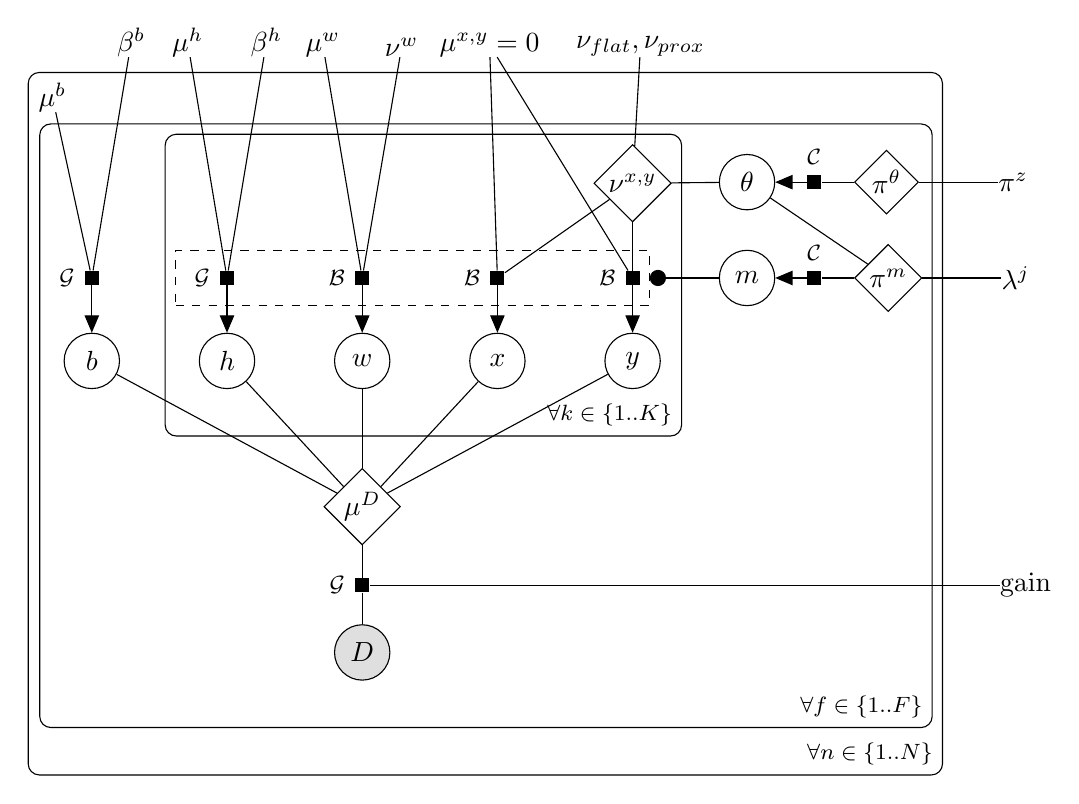
\begin{tikzpicture}

  % Define nodes

  % Y
  \node[obs]          (D)   {$D$}; %

  % W and X
  \node[det, above=of D]            (md) {$\mu^D$} ; % 
  \node[latent, above=of md] (w)   {$w$}; %
  \node[latent, above=of md, left=of w]  (h)   {$h$}; %
  \node[latent, above=of md, left=of h]  (b)   {$b$}; %
  \node[latent, above=of md, right=of w]  (x)   {$x$}; %
  \node[latent, above=of md, right=of x] (y)   {$y$}; %

  % b hyperparameters
  \node[const, above=2.8 of b, xshift=-0.5cm] (mb) {$\mu^b$} ; %
  \node[const, above=3.5 of b, xshift=0.5cm]  (bb) {$\beta^b$} ; %

  % h hyperparameters
  \node[const, above=3.5 of h, xshift=-0.5cm] (mh) {$\mu^h$} ; %
  \node[const, above=3.5 of h, xshift=0.5cm]  (bh) {$\beta^h$} ; %

  % w hyperparameters
  \node[const, above=3.5 of w, xshift=-0.5cm] (mw) {$\mu^w$} ; %
  \node[const, above=3.5 of w, xshift=0.5cm]  (nw) {$\nu^w$} ; %

  % xy hyperparameters
  \node[const, above=3.5 of x, xshift=-0.1cm] (mxy) {$\mu^{x,y}=0$} ; %
  \node[const, above=3.5 of y, xshift=0.1cm] (pr) {$\nu_{flat},\nu_{prox}$} ; %
  \node[det, above=1.4 of y]  (nxy) {$\nu^{x,y}$} ; %

  % Factors
  \factor[above=of D] {D-f} {left:$\mathcal{G}$} {} {} ; %
  \factor[above=0.6 of b] {b-f} {left:$\mathcal{G}$} {mb,bb} {b} ; %
  \factor[above=0.6 of h] {h-f} {left:$\mathcal{G}$} {mh,bh} {h} ; %
  \factor[above=0.6 of w] {w-f} {left:$\mathcal{B}$} {mw,nw} {w} ; %
  \factor[above=0.6 of x] {x-f} {left:$\mathcal{B}$} {mxy,nxy} {x} ; %
  \factor[above=0.6 of y] {y-f} {left:$\mathcal{B}$} {mxy,nxy} {y} ; %

  % D hyperparameters
  \node[const, right=8 of D-f] (g) {gain} ; %

  % m and theta
  \node[latent, right=of y-f] (m)   {$m$}; %
  \node[latent, above=0.5 of m] (t)   {$\theta$}; %

  % m and theta hyperparameters
  \node[det, right=1. of m]        (pm) {$\pi^m$} ; %
  \node[det, right=1. of t]        (pt) {$\pi^\theta$} ; %
  \node[const, right=of pt] (pz) {$\pi^z$} ; %
  \node[const, right=of pm] (lj) {$\lambda^j$} ; %

  % theta hyperparameters
  %\node[const, right=1.2 of t] (pt) {$\pi^\theta(\pi^z,\lambda^j)$} ; %

  % noise
  %\node[latent, right=2.5cm of y-f]         (t)   {$\tau$}; %
  %\node[const, above=of t, xshift=-0.5cm] (at)  {$\alpha_\tau$} ; %
  %\node[const, above=of t, xshift=0.5cm]  (bt)  {$\beta_\tau$} ; %

  % Factors
  \factor[right=of m] {m-f} {above:$\mathcal{C}$} {pm} {m} ; %
  \factor[right=of t] {t-f} {above:$\mathcal{C}$} {pt} {t} ; %
  %\factor[above=of x] {x-f} {left:$\mathcal{N}$} {mx,ax} {x} ; %
  %\factor[above=of t] {t-f} {left:$\mathcal{G}$} {at,bt} {t} ; %
  %\factoredge {dot,t} {y-f} {y} ; %

  \gate {m-gate} {(h-f)(h-f-caption)(h-f)(h-f-caption)(w-f)(w-f-caption)(x-f)(x-f-caption)(y-f)(y-f-caption)} {m}

  % Connect w and x to the dot node
  \factoredge[-] {g,md} {D-f} {D} ;
  \edge[-] {b,h,w,x,y} {md} ;
  \edge[-] {pz} {pt} ;
  \edge[-] {lj,t} {pm} ;
  \edge[-] {t,pr} {nxy} ;

  % Plates
  \plate {K} { %
    (h)(h-f)(h-f-caption) %
    (w)(w-f)(w-f-caption) %
    (x)(x-f)(x-f-caption) %
    (y)(y-f)(y-f-caption) %
    (m-gate) %
    (nxy)
  } {$\forall k \in \{ 1..K \}$} ;
  \plate {F} { %
    (K)
    (t)(t-f)(t-f-caption)(pt) %
    (m)(m-f)(m-f-caption)(pm) %
    (b)(b-f)(b-f-caption) %
    (md) %
    (D)(D-f)(D-f-caption) %
  } {$\forall f \in \{ 1..F \}$} ;
  \plate {N} { %
    (F)
    (mb)
  } {$\forall n \in \{ 1..N \}$} ;
  %\plate {} {%
    %(y)(y-f)(y-f-caption) %
    %(w)(w-f)(w-f-caption) %
    %(dot) %
    %(yx.north west)(yx.south west) %
  %} {$M$} ;

\end{tikzpicture}
%\endpgfgraphicnamed

%%% Local Variables: 
%%% mode: tex-pdf
%%% TeX-master: "example"
%%% End: 


  \end{center}
  \caption{Graphical model for the Bayesian classification model used in Pyro. The model has a modular structure consisting of three parts: classifier, the spot model, and the noise model. Hidden variables (circles) - background intensity ($b$), integrated intensity of the spot ($h$), width of the spot ($w$), position of the spot on the $x$-axis ($x$) and on the $y$-axis ($y$), existence indicator of spots ($m$), and index of the on-target spot ($\theta$). Observed variable (shaded circle) - image of the area of interest ($D$). Variables nested in plates are repeated for a number of times displayed at the bottom-right corner - target sites ($N$), frame count ($F$), number of spots in a single image ($K$). Densities are depicted as  small filled boxes. Deterministic functions are depicted as diamonds. Constants and hyperparameters are written without any borders. Gate (dashed box) represents variable activation conditioned on another variable.}
  \label{fig:graph}
\end{figure}

\subsection{Bayesian inference}

Probabilistic (Bayesian) model defines statistical relationship between hidden (unknown) and observed variables through a joint probability. In the case of CoSMoS experiment, unknown variables include global variables such as average probability of detecting a spot ($\pi^z$) and local variables like background intensity ($b_{nf}$) and the presence ($\theta_{nf}$), intensity ($h_{nfk}$), position ($x_{nfk}, y_{nfk}$), and width ($w_{nfk}$) of the spot. Observed variables are cropped 2D-images centered at target positions ($D_{nf}$). The structure and conditional independencies in the model can be represented as a factorization of the joint probability.

\textbf{\begin{equation*}
    p(b,\theta,m,h,w,x,y,pi^z,pi^j,D) = p(b)p(\theta|\pi^z)p(m|\theta,\pi^j)p(h|m)p(w)p(x|\theta)p(y|\theta)p(D|b,h,w,x,y)
\end{equation*}}


Alternatively, factorization of the joint probability can be visualized as a factor graph (Figure \ref{fig:graph}). In this graph, circular nodes represent random variables and solid square nodes represent probability distributions.

Bayesian inference is a statistical inference method that utilizes Bayes' theorem to update the probability of unknown variables conditional on observed data.

\subsection{Bayesian inference}

Probabilistic (Bayesian) model defines statistical relationship between hidden (unknown) and observed variables through a joint probability. In the case of CoSMoS experiment, unknown variables include global variables such as average probability of detecting a spot ($\pi^z$) and local variables like background intensity ($b_{nf}$) and the presence ($\theta_{nf}$), intensity ($h_{nfk}$), position ($x_{nfk}, y_{nfk}$), and width ($w_{nfk}$) of the spot. Observed variables are cropped 2D-images centered at target positions ($D_{nf}$). The structure and conditional independencies in the model can be represented as a factorization of the joint probability.

\textbf{\begin{equation*}
    p(b,\theta,m,h,w,x,y,pi^z,pi^j,D) = p(b)p(\theta|\pi^z)p(m|\theta,\pi^j)p(h|m)p(w)p(x|\theta)p(y|\theta)p(D|b,h,w,x,y)
\end{equation*}}

Alternatively, factorization of the joint probability can be visualized as a factor graph (Figure \ref{fig:graph}). In this graph, circular nodes represent random variables and solid square nodes represent probability distributions.

Bayesian inference is a statistical inference method that utilizes Bayes' theorem to update the probability of unknown variables conditional on observed data.

\textbf{\begin{equation*}
    p(b,\theta,m,h,w,x,y,pi^z,pi^j|D) = 
    \dfrac{p(b,\theta,m,h,w,x,y,pi^z,pi^j,D)}{p(D)}
\end{equation*}}

Bayesian inference seeks to determine the probability of a set of unknown
variables in light of a set of observed data. In the context of single-molecule
studies, these unknown variables are a set of model parameters q and a state
sequence zt, whereas the observations are a signal trajectory, xt. A graphical
model defines a statistical relationship between these variables that can
commonly be factored into two terms

The two distributions pðxjz; qÞ and pðz; qjj0Þ, known as the likelihood and
prior distribution, respectively, describe our assumptions about the model.
The likelihood describes the measurement signal we expect to see given
the state trajectory, zt, of the molecule and a set of emission model parameters that describe the distribution of measurement values associated
with each state. The prior distribution encodes our expectations about the
transition probabilities and emission model parameters. Based on these assumptions, the goal of Bayesian inference is now to reason about the socalled posterior probability of the state trajectory (zt) and model parameters
(q) in light of a set of measurements (xt). Bayes’ rule states that this posterior probability pðz; qjx; jÞ can be expressed as

\subsubsection{Noise model (The likelihood function)}

A model for CoSMoS data should capture several important aspects of co-localization process. The discrete hidden state of the observable image is a function of the total number of spots in the image and index of the on-target spot. The state probability is independent for each image.

\begin{equation*}
    \theta_{nf} \sim Categorical(\pi^z)
    m_{nf} \sim Categorical(\lambda, \theta)
\end{equation*}

Intensity of the spot is a function of the hidden state. Position prior is the function of the hidden state. Local background intensity.

\subsubsection{Image model}

In the TIBSD method, we model the observed image data as a mixture of background image and “spot” images of binder molecules superimposed on background image. In particular, background image is modeled as a constant average background intensity $b_{nf}$; each spot image (2D point spread function) is modelled as an ideal (i.e., noiseless) 2-D Gaussian spot with integrated scalar intensity $h_{nfk}$ centered at ($x_{nfk}, y_{nfk}$).  

\textbf{\begin{equation*}
    \mu^{D}_{nfij} = b_{nf} + \sum_{k=1}^{K} \dfrac{h_{nfk}}{2 \pi w^2_{nfk}} \exp{\left ( -\dfrac{(i-x_{nfk})^2 + (j-y_{nfk})^2}{2w^2_{nfk}} \right)}
\end{equation*}}

We use Gamma distribution as a noise model which is more flexible than Gaussian noise and can better approximate Poissonian camera noise. Scale parameter [add the variable name here?] of the Gamma distribution can be interpreted as a camera gain. Thus, the likelihood for the observed image can be expressed as:
 
 \begin{equation*}
     p(D_{nf}|\mu^D_{nfij},gain) = Gamma(D_{nf}|\mu^D_{nfij}/gain,1/gain)
 \end{equation*}

Stochastic variational inference.

\subsection{Time-independent Bayesian Spot Discrimination (TIBSD) method for analysis of CoSMoS data}

Unlike standard analysis methods for CoSMoS and single molecule FRET (smFRET), which are based on scalar intensity measurements derived from integration of emission in image regions of interest, our model fully uses information contained in the raw two-dimensional microscope images. The value of image data is proven in previous studies \citep{Friedman2015-nx,Smith2019-yb}. To analyze the CoSMoS image classification problem within a Bayesian framework, one must define ideal image shapes for each class (image model) and choose a likelihood function for the observed data (noise model).

In each image, a binder molecule is either present on the single target molecule or absent. In addition, we explicitly model off-target binding of binder molecule. For simplicity  we assume that experimental conditions and image size were chosen so that at most only two spots ($K=2$) can exist in one image ($m_{nfk} \in \{ 0,1 \}$ -- existence indicator of the $k$-th spot). We treat the image classification problem as a data association problem by introducing an index variable for the on-target spot ($\theta_{nf} \in \{ 0,1,\dots,K \}$) where 0 means that on-target molecule is absent.





\subsubsection{Prior knowledge of colocalization accuracy}

Prior knowledge of colocalization accuracy can be directly incorporated into our model as priors for the center of the spot. On-target spots are localized around the target molecule within the experimentally determined accuracy and off-target spots are uniformly distributed within the image:

\begin{equation*}
    x_{nfk} \sim
\begin{cases}
    Beta^{\prime}(x_{nfk}|\mu^x=0,\nu^x_{prox}),& \text{if } \theta = k\\
    Beta^{\prime}(x_{nfk}|\mu^x=0,\nu^x_{flat}),& \text{otherwise}
\end{cases}
\end{equation*}

\begin{equation*}
    y_{nfk} \sim
\begin{cases}
    Beta^{\prime}(y_{nfk}|\mu^y=0,\nu^y_{prox}),& \text{if } \theta = k\\
    Beta^{\prime}(y_{nfk}|\mu^y=0,\nu^y_{flat}),& \text{otherwise}
\end{cases}
\end{equation*}


%\subsection{Image analysis, probabilities not binary classification}

%Expresses uncertainty. Allows downstream analysis. 

%\subsection{Flexible framework. Can select and use different models depending on the experiment}

%\subsubsection{Ability to jointly analyze different experimental conditions}

%\subsubsection{Models easily expandable to incorporate other data features}

\subsection{Software and hardware implementation}

The proposed research will provide more efficient ways to analyze large CoSMoS data sets. Technological developments such as faster, larger cameras \citep{Quan2011-cg}, availability of fluorescent dyes with dramatically improved photostability (which increase the amount of data from a single experiment), and microscopes that efficiently collect single-molecule data at more wavelengths simultaneously \citep{Friedman2006-kb} have all increased the sizes of CoSMoS datasets. Gelles lab studies of transient molecular binding events at high frame rates have produced >1 TB image data per experiment. Increasing data set sizes make it infeasible to use existing analytical methods. The code for the model and variational inference algorithm is written using Pyro probabilistic programming language. Pyro uses Pytorch as a backend for automatic differentiation and efficient computation of parallelizable vector-math operations on graphics processing units (GPUs). Our program is open-source and can be downloaded from the github repository.

\begin{comment}
\begin{table}[bt]
\caption{\label{tab:example}Automobile Land Speed Records (GR 5-10).}
% Use "S" column identifier to align on decimal point 
\begin{tabular}{S l l l r}
\toprule
{Speed (mph)} & Driver          & Car                        & Engine    & Date     \\
\midrule
407.447     & Craig Breedlove & Spirit of America          & GE J47    & 8/5/63   \\
413.199     & Tom Green       & Wingfoot Express           & WE J46    & 10/2/64  \\
434.22      & Art Arfons      & Green Monster              & GE J79    & 10/5/64  \\
468.719     & Craig Breedlove & Spirit of America          & GE J79    & 10/13/64 \\
526.277     & Craig Breedlove & Spirit of America          & GE J79    & 10/15/65 \\
536.712     & Art Arfons      & Green Monster              & GE J79    & 10/27/65 \\
555.127     & Craig Breedlove & Spirit of America, Sonic 1 & GE J79    & 11/2/65  \\
576.553     & Art Arfons      & Green Monster              & GE J79    & 11/7/65  \\
600.601     & Craig Breedlove & Spirit of America, Sonic 1 & GE J79    & 11/15/65 \\
622.407     & Gary Gabelich   & Blue Flame                 & Rocket    & 10/23/70 \\
633.468     & Richard Noble   & Thrust 2                   & RR RG 146 & 10/4/83  \\
763.035     & Andy Green      & Thrust SSC                 & RR Spey   & 10/15/97\\
\bottomrule
\end{tabular}

\medskip 
Source: \url{https://www.sedl.org/afterschool/toolkits/science/pdf/ast_sci_data_tables_sample.pdf}

\tabledata{This is a description of a data source.}

\end{table}
\end{comment}

%\section{Some \LaTeX{} Examples}
\label{sec:examples}

Use section and subsection commands to organize your document. \LaTeX{} handles all the formatting and numbering automatically. Use ref and label commands for cross-references.

\subsection{Figures and Tables}

Use the table and tabular commands for basic tables --- see \TABLE{example}, for example. 

You can upload a figure (JPEG, PNG or PDF) using the project menu. To include it in your document, use the \verb|\includegraphics| command as in the code for \FIG{view}. 

For a half-width figure or table with text wrapping around it, use 

\begin{verbatim}
\begin{wrapfigure}{l}{.46\textwidth}
  \includegraphics[width=\hsize]{...}
  \caption{...}\label{...}
\end{wrapfigure}
\end{verbatim}
%
as in \FIG{halfwidth}. For tables:

\begin{verbatim}
\begin{wraptable}{l}{.46\textwidth}{
  \begin{tabular}{...}
  ...
  \end{tabular}}
  \caption{...}\label{...}
\end{wraptable}
\end{verbatim}

Be careful with these, though, as they may behave strangely near page boundaries, sectional headings, or in the neighbourhood of lists or too many floats.

Labels for main videos can be added with \verb|\video| e.g.

\video{Ths is a description of a main video.}\label{video:mv1}
\video{Another!}

Labels for video supplements can be added within \texttt{figure} environments, after the \texttt{caption}, using the \verb|\videosupp| command: see \VIDEOSUPP[view]{sv1} for an example.

If you use the following prefixes for your \verb|\label|:
%
\begin{description}
\item[Figures] \texttt{fig:}, e.g.~\verb|\label{fig:view}|
\item[Figure Supplements] \texttt{figsupp:}, e.g.~\verb|\label{figsupp:sf1}|\\
(we'll assume \texttt{figsupp:sf1} is a figure supplement of \texttt{fig:view} in our example)
\item[Figure source data] \texttt{figdata:}, e.g.~\verb|\label{figdata:first}|
\item[Videos] \texttt{video:}, e.g.~\verb|\label{video:mv1}|
\item[Video supplements] \texttt{videosupp:}, e.g.~\verb|\label{videosupp:sv1}|
\item[Tables] \texttt{tab:}, e.g.~\verb|\label{tab:example}|
\item[Equations] \texttt{eq:}, e.g.~\verb|\label{eq:CLT}|
\item[Boxes] \texttt{box:}, e.g.~\verb|\label{box:simple}|
\end{description}
%
you can then use the convenience commands \verb|\FIG{view}|, \verb|\FIGSUPP[view]{sf1}|, \verb|\TABLE{example}|, \verb|\EQ{CLT}|, \verb|\BOX{simple}|, \verb|\FIGDATA[view]{first}|, \verb|\VIDEO{mv1}| and \verb|{\VIDEOSUPP}[view]{sv1}| \emph{without} the label prefixes, to generate cross-references \FIG{view}, \FIGSUPP[view]{sf1},  \TABLE{example}, \EQ{CLT}, \BOX{simple}, \FIGDATA[view]{first}, \VIDEO{mv1} and \VIDEOSUPP[view]{sv1}. Alternatively, use \verb|\autoref| with the full label, e.g.~\autoref{first:app} (although this may not work correctly for figures and tables in the appendices or boxes nor supplements at present).

Really wide figures or tables, that take up the entire page, including the gutter space: use \verb|\begin{fullwidth}...\end{fullwidth}| as in \FIG{fullwidth}. And sometimes you may want to use feature boxes like \BOX{simple}.

\begin{wrapfigure}{l}{.46\textwidth}
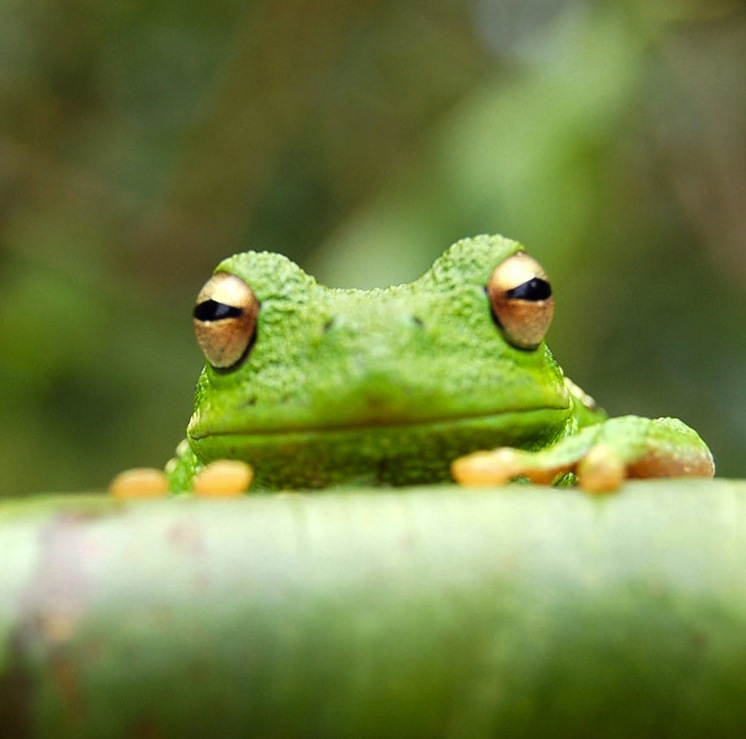
\includegraphics[width=\hsize]{frog}
\caption{A half-columnwidth image using wrapfigure, to be used sparingly. Note that using a wrapfigure before a sectional heading, near other floats or page boundaries is not recommended, as it may cause interesting layout issues. Use the optional argument to wrapfigure to control how many lines of text should be set half-width alongside it.}
\label{fig:halfwidth}
\end{wrapfigure}

Some filler text to sit alongside the half-width figure. \lipsum[1-2]

\begin{figure}
\begin{fullwidth}
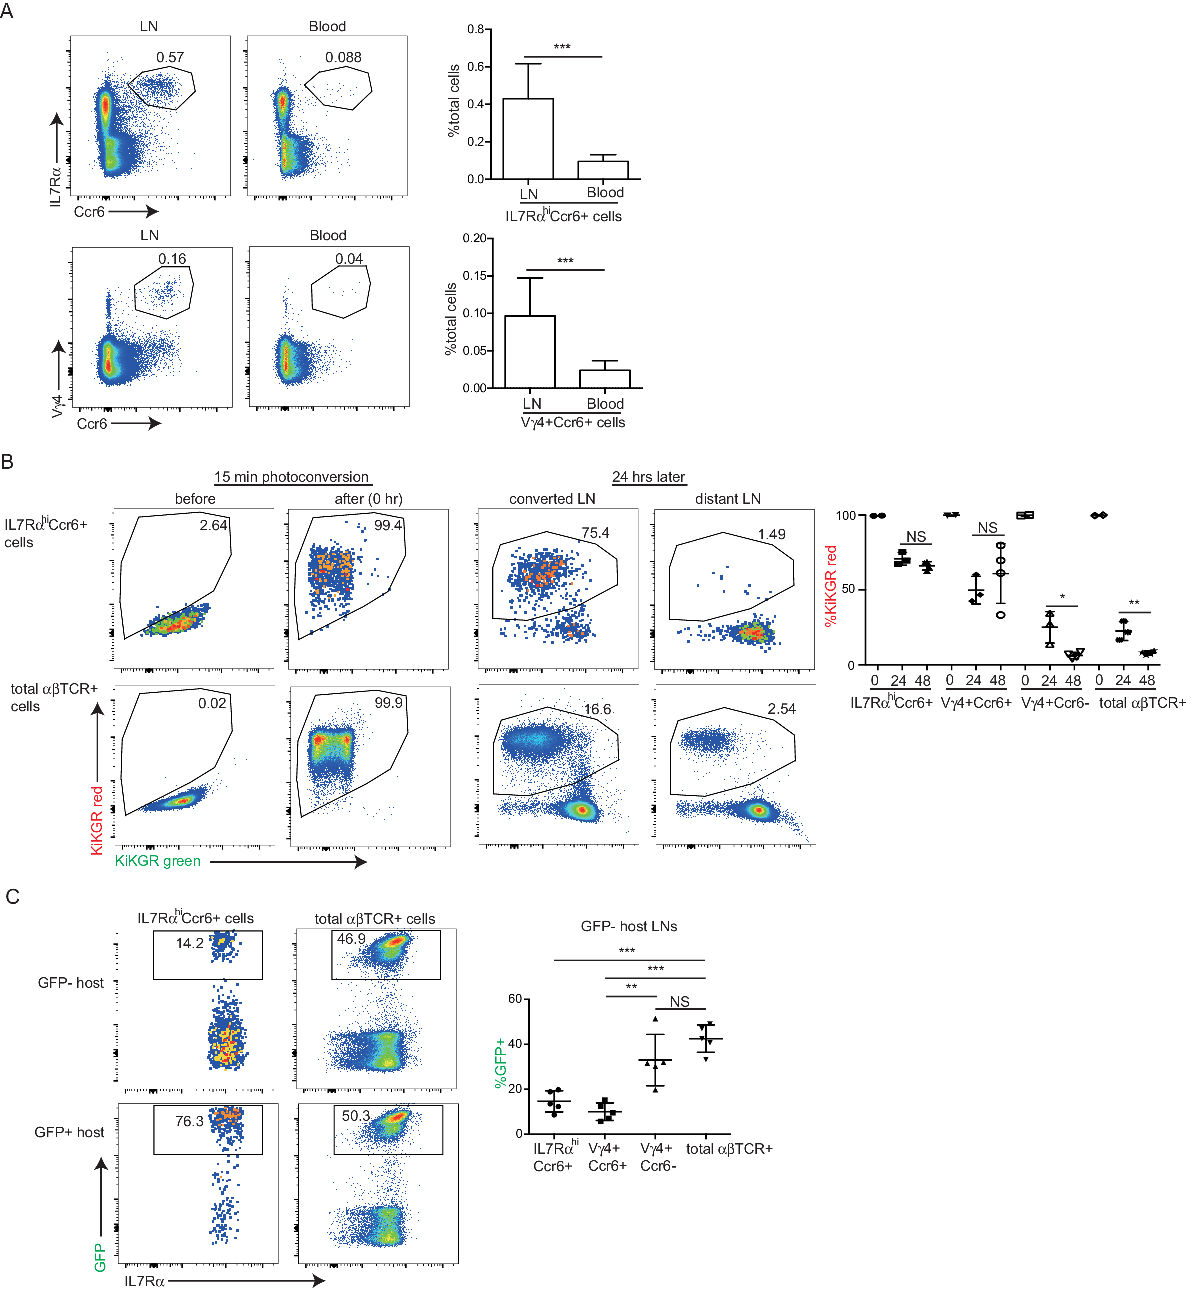
\includegraphics[width=0.95\linewidth]{elife-18156-fig2}
\caption{A very wide figure that takes up the entire page, including the gutter space.}
\label{fig:fullwidth}
\figsupp{There is no limit on the number of Figure Supplements for any one primary figure. Each figure supplement should be clearly labelled, Figure 1--Figure Supplement 1, Figure 1--Figure Supplement 2, Figure 2--Figure Supplement 1 and so on, and have a short title (and optional legend). Figure Supplements should be referred to in the legend of the associated primary figure, and should also be listed at the end of the article text file.}{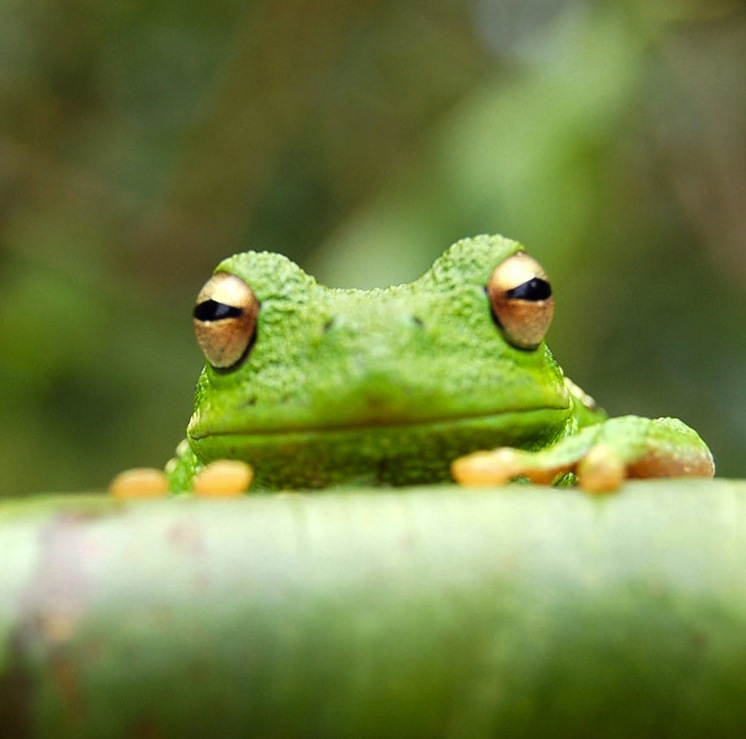
\includegraphics[width=5cm]{frog}}
\end{fullwidth}
\end{figure}

\subsection{Citations}

LaTeX formats citations and references automatically using the bibliography records in your .bib file, which you can edit via the project menu. Use the \verb|\cite| command for an inline citation, like \cite{Aivazian917}, and the \verb|\citep| command for a citation in parentheses \citep{Aivazian917}. The LaTeX template uses a slightly-modified Vancouver bibliography style. If your manuscript is accepted, the eLife production team will re-format the references into the final published form. \emph{It is not necessary to attempt to format the reference list yourself to mirror the final published form.} Please also remember to \textbf{delete the line} \verb|\nocite{*}| in the template just before \verb|\bibliography{...}|; otherwise \emph{all} entries from your .bib file will be listed! 

\begin{featurebox}
\caption{This is an example feature box}
\label{box:simple}
This is a feature box. It floats!
\medskip

\includegraphics[width=5cm]{example-image}
\featurefig{`Figure' and `table' captions in feature boxes should be entered with \texttt{\textbackslash featurefig} and \texttt{\textbackslash featuretable}. They're not really floats.}

\lipsum[1]
\end{featurebox}

\subsection{Mathematics}

\LaTeX{} is great at typesetting mathematics. Let $X_1, X_2, \ldots, X_n$ be a sequence of independent and identically distributed random variables with $\text{E}[X_i] = \mu$ and $\text{Var}[X_i] = \sigma^2 < \infty$, and let
\begin{equation}
\label{eq:CLT}
S_n = \frac{X_1 + X_2 + \cdots + X_n}{n}
      = \frac{1}{n}\sum_{i}^{n} X_i
\end{equation}
denote their mean. Then as $n$ approaches infinity, the random variables $\sqrt{n}(S_n - \mu)$ converge in distribution to a normal $\mathcal{N}(0, \sigma^2)$.

\lipsum[3] 

\begin{figure}
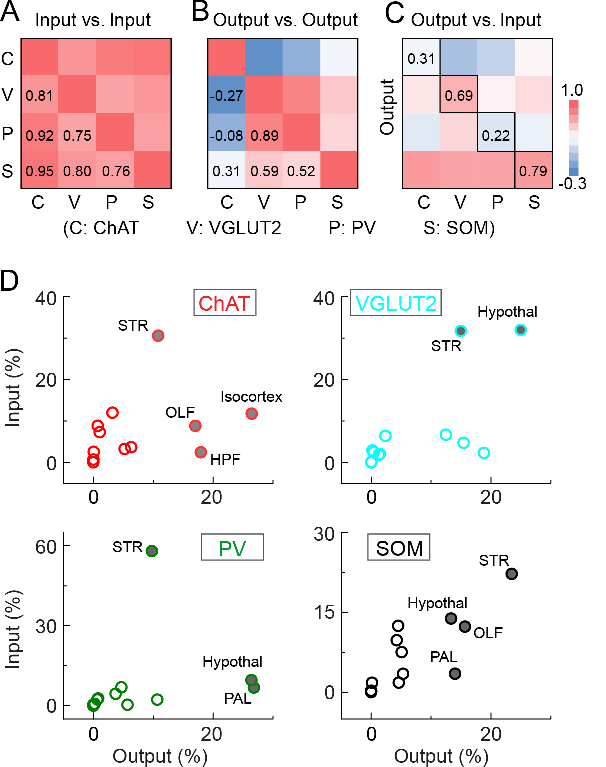
\includegraphics[width=\linewidth]{elife-13214-fig7}
\caption{A text-width example.}
\label{fig:view}
%% If the optional argument in the square brackets is "none", then the caption *will not appear in the main figure at all* and only the full caption will appear under the supplementary figure at the end of the manuscript.
\figsupp[Shorter caption for main text.]{This is a supplementary figure's full caption, which will be used at the end of the manuscript.}{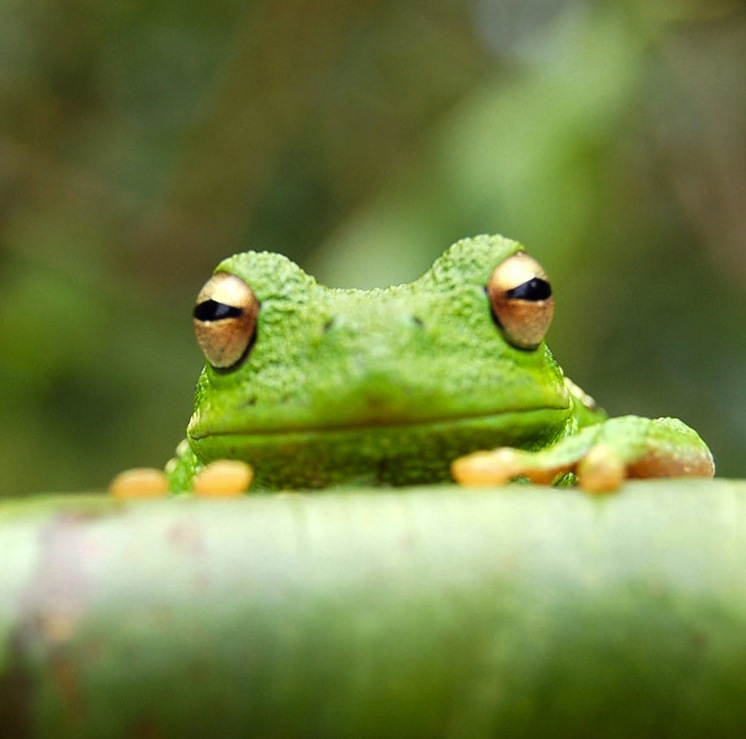
\includegraphics[width=6cm]{frog}}\label{figsupp:sf1}
\figsupp{This is another supplementary figure.}{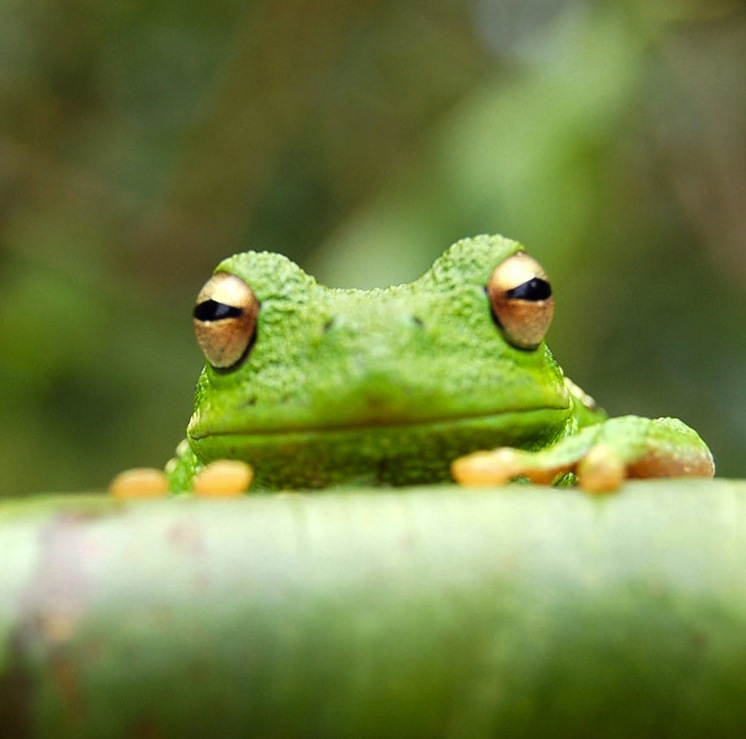
\includegraphics[width=6cm]{frog}}
\videosupp{This is a description of a video supplement.}\label{videosupp:sv1}
\figdata{This is a description of a data source.}\label{figdata:first}
\figdata{This is another description of a data source.}\label{figdata:second}
\end{figure}

\subsection{Other Chemistry Niceties}

You can use commands from the \texttt{mhchem} and \texttt{siunitx} packages. For example: \ce{C32H64NO7S}; \SI{5}{\micro\metre}; \SI{30}{\degreeCelsius}; \SI{5e-17}{\Molar}

\subsection{Lists}

You can make lists with automatic numbering \dots

\begin{enumerate}
\item Like this,
\item and like this.
\end{enumerate}
\dots or bullet points \dots
\begin{itemize} 
\item Like this,
\item and like this.
\end{itemize}
\dots or with words and descriptions \dots
\begin{description}
\item[Word] Definition
\item[Concept] Explanation
\item[Idea] Text
\end{description}

Some filler text, because empty templates look really poorly. \lipsum[1]

%\section{Acknowledgments}

Additional information can be given in the template, such as to not include funder information in the acknowledgments section.

%\nocite{*} % This command displays all refs in the bib file. PLEASE DELETE IT BEFORE YOU SUBMIT YOUR MANUSCRIPT!
\bibliography{references}

%\section{Supplementary Material}

\subsection{Variable definitions}

Target site
\begin{equation*}
    n \in \{1,\dots,N\}
\end{equation*}
%
Frame number
\begin{equation*}
    f \in \{1,\dots,F\}
\end{equation*}
%
$x$-axis pixel number
\begin{equation*}
    i \in \{1,\dots,I\}
\end{equation*}
%
$y$-axis pixel number
\begin{equation*}
    j \in \{1,\dots,J\}
\end{equation*}
%
Spot index
\begin{equation*}
    k \in \{1,\dots,K\}
\end{equation*}
%
Background intensity
\begin{equation*}
    b_{nf} > 0
\end{equation*}
%
Hidden state
\begin{equation*}
    m_{nf}
\end{equation*}
%
Integrated spot intensity
\begin{equation*}
    h_{nfk} > 0
\end{equation*}
%
Ideal spot shape
\begin{equation*}
    \mu^{D}_{nfij} = b_{nf} + \sum_k \dfrac{m_{nfk}h_{nfk}}{2 \pi w^2_{nfk}} \exp{\left ( -\dfrac{(i-x_{nfk})^2 + (j-y_{nfk})^2}{2w^2_{nfk}} \right)}
\end{equation*}

\end{document}
